\documentclass[11pt,a4paper]{report}

% ══════════════════════════════════════════════════════════════════════
%  X5 — Documento extendido. Compilar con: tectonic x5_documento_extendido.tex
%  Motor XeTeX (UTF-8 nativo). Fusiona y amplía x5_plan.md + x5_plan_redes_neuronales.md
% ══════════════════════════════════════════════════════════════════════

\usepackage{fontspec}
\usepackage{amsmath,amssymb}
\usepackage[margin=2.3cm]{geometry}
\usepackage{xcolor}
\usepackage{tikz}
\usetikzlibrary{positioning,arrows.meta,shapes.geometric,fit,backgrounds,calc,decorations.pathreplacing}
\usepackage{booktabs}
\usepackage{listings}
\usepackage{enumitem}
\usepackage{tcolorbox}
\usepackage{titlesec}
\usepackage[hidelinks]{hyperref}

% ── Nombres en español (sin babel para evitar choques con fontspec/tectonic) ──
\renewcommand{\chaptername}{Capítulo}
\renewcommand{\contentsname}{Índice}
\renewcommand{\tablename}{Tabla}
\renewcommand{\figurename}{Figura}
\renewcommand{\today}{\number\day\ de \ifcase\month\or enero\or febrero\or marzo\or
  abril\or mayo\or junio\or julio\or agosto\or septiembre\or octubre\or noviembre\or
  diciembre\fi\ de \number\year}

% ── Colores ──
\definecolor{cazul}{HTML}{2C5F8A}
\definecolor{cverde}{HTML}{2E8B57}
\definecolor{cnaranja}{HTML}{C1660A}
\definecolor{cgris}{HTML}{5B6770}
\definecolor{crojo}{HTML}{B23A48}
\definecolor{cfondo}{HTML}{F2F5F8}
\definecolor{ccode}{HTML}{F6F8FA}

% ── Títulos de capítulo compactos ──
\titleformat{\chapter}[display]
  {\normalfont\huge\bfseries\color{cazul}}
  {\chaptertitlename\ \thechapter}{16pt}{\Huge}
\titlespacing*{\chapter}{0pt}{-10pt}{24pt}

% ── Código ──
\lstset{
  basicstyle=\ttfamily\small,
  backgroundcolor=\color{ccode},
  frame=single, rulecolor=\color{cgris!40},
  breaklines=true, columns=fullflexible, keepspaces=true,
  showstringspaces=false, xleftmargin=6pt, framexleftmargin=4pt,
}
% \code permite partir nombres largos en los guiones bajos (evita overfull)
\newcommand{\code}[1]{\texttt{\def\_{\textunderscore\allowbreak}#1}}
\setlength{\emergencystretch}{3em}

% ── Caja de "idea clave" ──
\newtcolorbox{idea}[1][]{colback=cverde!6, colframe=cverde!55, boxrule=0.6pt,
  arc=2pt, left=6pt, right=6pt, top=4pt, bottom=4pt, fonttitle=\bfseries, title={#1}}
\newtcolorbox{ejemplo}[1][]{colback=cnaranja!6, colframe=cnaranja!55, boxrule=0.6pt,
  arc=2pt, left=6pt, right=6pt, top=4pt, bottom=4pt, fonttitle=\bfseries, title={#1}}
\newtcolorbox{nota}[1][]{colback=cgris!8, colframe=cgris!50, boxrule=0.6pt,
  arc=2pt, left=6pt, right=6pt, top=4pt, bottom=4pt, fonttitle=\bfseries, title={#1}}

% ── Estilos TikZ ──
\tikzset{
  caja/.style={rectangle, rounded corners=3pt, draw=cazul, fill=cazul!8,
    text width=2.9cm, align=center, minimum height=1cm, font=\small},
  cajav/.style={rectangle, rounded corners=3pt, draw=cverde, fill=cverde!8,
    text width=2.9cm, align=center, minimum height=1cm, font=\small},
  cajan/.style={rectangle, rounded corners=3pt, draw=cnaranja, fill=cnaranja!8,
    text width=2.9cm, align=center, minimum height=1cm, font=\small},
  cajar/.style={rectangle, rounded corners=3pt, draw=crojo, fill=crojo!8,
    text width=2.9cm, align=center, minimum height=1cm, font=\small},
  cajag/.style={rectangle, rounded corners=3pt, draw=cgris, fill=cgris!8,
    text width=2.5cm, align=center, minimum height=0.9cm, font=\small},
  flecha/.style={-{Stealth[length=3mm]}, thick, draw=cgris},
  etq/.style={font=\footnotesize\itshape, text=cgris},
}
\newcommand{\diag}[1]{\begin{center}\resizebox{\textwidth}{!}{#1}\end{center}}

% ══════════════════════════════════════════════════════════════════════
\begin{document}

\begin{titlepage}
\centering
\vspace*{2.5cm}
{\Huge\bfseries\color{cazul} X5 — El cerebro de Alginvesting\par}
\vspace{0.6cm}
{\Large Surrogate model para el ajuste dinámico de parámetros de trading\par}
\vspace{0.4cm}
{\large\color{cgris} Versión extendida — guía técnica y conceptual completa\par}
\vspace{2cm}
\begin{minipage}{0.8\textwidth}\color{cgris}\small\itshape
Documento de referencia para entender X5 de principio a fin: qué hace, por qué,
cómo está construido (Gradient Boosting y FT-Transformer), cómo se entrena desde
cero con backtesting paralelo, cómo recomienda los parámetros óptimos y cómo se
integra al sistema. Explicado con analogías y ejemplos numéricos, pensado para
leerse impreso sin necesidad de consultar el código.
\end{minipage}
\vfill
{\color{cgris} Proyecto Alginvesting \quad\textbullet\quad \today}
\end{titlepage}

\tableofcontents
\thispagestyle{empty}

% ══════════════════════════════════════════════════════════════════════
\chapter{Introducción: qué es X5 y por qué es el cerebro}

\section{El sistema en 30 segundos}

Alginvesting es un sistema de trading algorítmico que opera comprando en \textbf{soportes}
(niveles de precio donde históricamente el precio ``rebota''). El sistema tiene varios módulos:

\begin{center}
\begin{tabular}{@{}ll@{}}
\toprule
\textbf{Módulo} & \textbf{Qué hace} \\
\midrule
X0 & Descarga precios y calcula los soportes óptimos. \\
X1 & Coloca y gestiona las órdenes en vivo (buy limits, trailing stop, cierres). \\
X2 & Calcula un score fundamental por activo (¿está sano el activo?). \\
X3 & Calcula features técnicas por activo (RSI, medias móviles, volatilidad\ldots). \\
X4 & Backtester: simula X1 sobre la historia para probar configuraciones. \\
\textbf{X5} & \textbf{El cerebro: decide qué parámetros usar según el mercado.} \\
\bottomrule
\end{tabular}
\end{center}

Todos esos módulos dependen de un conjunto de \textbf{parámetros de configuración}. Hoy esos
parámetros son fijos (los define una persona en \code{config.py}). El problema es que los
parámetros \emph{óptimos no son siempre los mismos}: dependen del estado del mercado.

\begin{idea}[La idea central]
Cuando el mercado cambia de ``personalidad'' (de alcista a bajista, de calmado a volátil),
los parámetros que eran buenos dejan de serlo. \textbf{X5 es el módulo que ajusta esos
parámetros automáticamente, según cómo está el mercado en cada momento.} Por eso es el cerebro.
\end{idea}

\section{Los parámetros que X5 controla}

\begin{center}
\small
\begin{tabular}{@{}llp{7.3cm}@{}}
\toprule
\textbf{Parámetro} & \textbf{Tipo} & \textbf{Qué hace} \\
\midrule
\code{n\_sizes\_ejecucion} & int & Cuántos soportes activos mantener por activo. \\
\code{K} & float & Peso del aislamiento futuro vs.\ pasado en el scoring de soportes. \\
\code{N\_EXP} & float & Exponente de recencia (cuánto pesan las velas recientes). \\
\code{LAMBDA} & float & Penaliza que los soportes se amontonen en una zona del rango. \\
\code{A} & float & Ganancia mínima (USD) para activar el primer trailing stop. \\
\code{B} & float & Holgura (USD) que el trailing stop mantiene bajo el precio. \\
\code{LOTAJES\_M} & int & Multiplicador de lote (tamaño de cada posición). \\
\code{PERDIDA\_MAX} & float & Pérdida máxima (USD) por posición antes de cerrarla. \\
\bottomrule
\end{tabular}
\end{center}

\begin{nota}[Todo es por activo]
X5 no entrena un solo modelo global. Entrena \textbf{un modelo independiente por activo}
(BTCUSD, ETHUSD, TSLA, GOOGL, NVDA, AMZN). BTC (muy volátil, 24/7) y GOOGL (más estable,
horario bursátil) tienen dinámicas distintas, así que sus parámetros óptimos difieren. Cada
activo tiene su propio cuaderno de datos, su propio modelo y su propio ritmo de aprendizaje.
\end{nota}

\section{El flujo completo}

\diag{
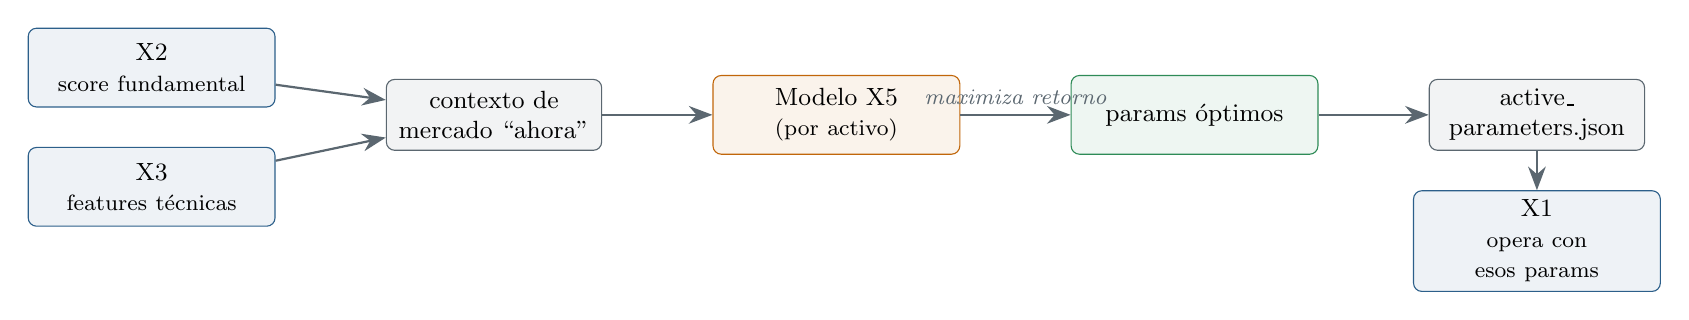
\begin{tikzpicture}[node distance=0.9cm and 1.4cm]
  \node[caja] (x2) {X2\\\footnotesize score fundamental};
  \node[caja, below=0.5cm of x2] (x3) {X3\\\footnotesize features técnicas};
  \node[cajag, right=of x2, yshift=-0.6cm] (ctx) {contexto de\\mercado ``ahora''};
  \node[cajan, right=of ctx] (modelo) {Modelo X5\\\footnotesize (por activo)};
  \node[cajav, right=of modelo] (params) {params óptimos};
  \node[cajag, right=of params] (json) {active\_\\parameters.json};
  \node[caja, below=0.5cm of json] (x1) {X1\\\footnotesize opera con esos params};
  \draw[flecha] (x2) -- (ctx);
  \draw[flecha] (x3) -- (ctx);
  \draw[flecha] (ctx) -- (modelo);
  \draw[flecha] (modelo) -- (params) node[midway,above,etq]{maximiza retorno};
  \draw[flecha] (params) -- (json);
  \draw[flecha] (json) -- (x1);
\end{tikzpicture}}

En una frase: \emph{X5 mira cómo está el mercado (X2 + X3), le pregunta a su modelo qué
parámetros darían el mejor retorno, y escribe la respuesta en un archivo que X1 puede leer.}

% ══════════════════════════════════════════════════════════════════════
\chapter{El problema que resuelve X5}

\section{Por qué los parámetros fijos no bastan}

Imagina que fijas \code{LOTAJES\_M = 3} (posiciones grandes) porque en un mercado alcista te dio
buenos resultados. Llega un \emph{crash}: el precio cae 15\% en dos días. Con posiciones grandes,
las pérdidas se multiplican. Un valor de \code{LOTAJES\_M = 1} habría sufrido mucho menos.

El problema no es que ``3'' esté mal. Es que \textbf{``3'' era bueno en un régimen y malo en
otro}. Ningún valor fijo es óptimo para todos los escenarios.

\begin{ejemplo}[Ejemplo numérico simple]
Supón dos posiciones abiertas en BTC con entrada en \$95.000, y el precio cae a \$88.000
($-7,4\%$). Con lote base que mueve \$1 por dólar de BTC:
\begin{itemize}[itemsep=1pt]
  \item \code{LOTAJES\_M = 1}: pérdida flotante $\approx 2 \times (88.000-95.000) \times 0{,}01 = -\$140$.
  \item \code{LOTAJES\_M = 3}: pérdida flotante $\approx 2 \times (88.000-95.000) \times 0{,}03 = -\$420$.
\end{itemize}
Mismo mercado, misma estrategia: solo cambiar un parámetro triplica la pérdida. Si X5 hubiera
detectado el régimen de caída y bajado \code{LOTAJES\_M} a 1 \emph{antes}, el daño sería un tercio.
\end{ejemplo}

\section{El enfoque: surrogate model + optimización en inferencia}

Un \textbf{surrogate model} (modelo sustituto) es un modelo que ``imita'' un sistema costoso de
evaluar para poder hacer predicciones baratas. En vez de esperar a que el mercado nos diga si
una configuración fue buena (lo cual toma semanas de trading real), entrenamos un modelo que
\emph{predice} el resultado.

El plan de X5 tiene dos mitades:

\begin{enumerate}[leftmargin=1.5em]
  \item \textbf{Entrenamiento} — se entrena un modelo que aprende la relación:
  \[
    f(\underbrace{\text{contexto X2+X3}}_{\text{cómo está el mercado}},\ \underbrace{\text{parámetros}}_{\text{qué configuración uso}}) \;\longrightarrow\; \underbrace{\text{retorno esperado}}_{\text{cuánto gano}}
  \]
  \item \textbf{Inferencia} — con el contexto de mercado \emph{fijo} (el de ahora), se busca el
  conjunto de parámetros que \textbf{maximiza} el retorno que el modelo predice. Ese conjunto se
  escribe en \code{config/active\_parameters.json}.
\end{enumerate}

\begin{idea}[La inversión clave]
El modelo aprende a \emph{predecir} el retorno dado (mercado, parámetros). Pero en inferencia lo
usamos ``al revés'': fijamos el mercado y \textbf{buscamos los parámetros} que producen el
retorno más alto. Es optimización sobre las entradas del modelo, no sobre sus pesos.
\end{idea}

% ══════════════════════════════════════════════════════════════════════
\chapter{La analogía del chef (el hilo conductor)}

A lo largo del documento usaremos una analogía. Vale la pena fijarla bien porque conecta todas
las piezas.

\begin{center}
\small
\begin{tabular}{@{}ll@{}}
\toprule
\textbf{En la analogía} & \textbf{En X5} \\
\midrule
El chef & El modelo de aprendizaje automático. \\
El cuaderno de recetas & El \emph{store} de datos (\code{\{ACTIVO\}\_store.csv}). \\
Una receta & Un conjunto de parámetros de configuración. \\
Cómo estaba la cocina ese día & El contexto de mercado (X2 + X3). \\
Cómo quedó el plato & El retorno de la operación (la variable objetivo). \\
Practicar cocinando & Generar datos con backtesting (\code{-{}-recolectar}). \\
Estudiar el cuaderno & Entrenar el modelo. \\
Pedir la mejor receta para hoy & Inferir los parámetros (\code{-{}-infer}). \\
\bottomrule
\end{tabular}
\end{center}

\noindent Un chef que cocinó miles de platos en cocinas de distintas condiciones puede predecir:
``con esta receta, en una cocina así, el plato sale 8/10''. Al principio, sin embargo, el chef
\textbf{no sabe nada}: hay que hacerlo cocinar mucho para llenar el cuaderno. Ese es
exactamente el estado actual de X5: el cuaderno está vacío, así que el primer trabajo es
generar datos.

% ══════════════════════════════════════════════════════════════════════
\chapter{Los datos: qué entra y qué sale del modelo}

\section{Panorama de los inputs (\textasciitilde240 columnas)}

Cada fila del cuaderno representa una operación (o un momento del portfolio). Sus columnas se
agrupan en cinco bloques, que juntos forman un vector de \textbf{tamaño fijo} (\textasciitilde240
números) que entra al modelo:

\diag{
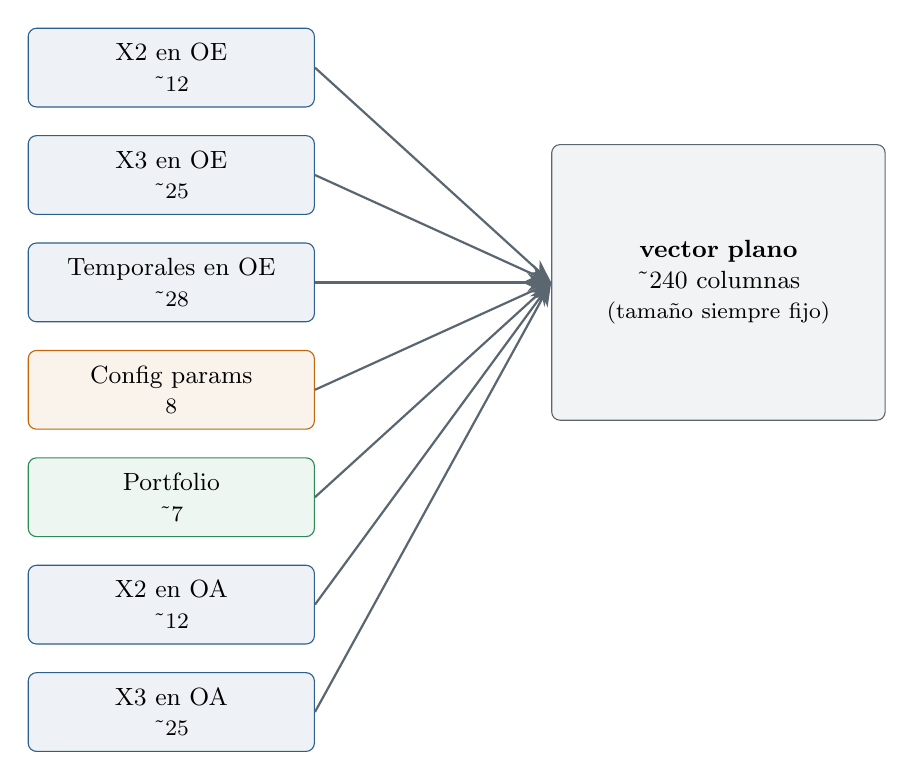
\begin{tikzpicture}[node distance=0.35cm]
  \node[caja, text width=3.4cm] (a) {X2 en OE\\\footnotesize \textasciitilde12};
  \node[caja, below=of a, text width=3.4cm] (b) {X3 en OE\\\footnotesize \textasciitilde25};
  \node[caja, below=of b, text width=3.4cm] (c) {Temporales en OE\\\footnotesize \textasciitilde28};
  \node[cajan, below=of c, text width=3.4cm] (d) {Config params\\\footnotesize 8};
  \node[cajav, below=of d, text width=3.4cm] (e) {Portfolio\\\footnotesize \textasciitilde7};
  \node[caja, below=of e, text width=3.4cm] (f) {X2 en OA\\\footnotesize \textasciitilde12};
  \node[caja, below=of f, text width=3.4cm] (g) {X3 en OA\\\footnotesize \textasciitilde25};
  \node[cajag, right=3cm of c, text width=4cm, minimum height=3.5cm] (vec)
    {\textbf{vector plano}\\\textasciitilde240 columnas\\\footnotesize (tamaño siempre fijo)};
  \draw[flecha] (a.east) -- (vec.west);
  \draw[flecha] (b.east) -- (vec.west);
  \draw[flecha] (c.east) -- (vec.west);
  \draw[flecha] (d.east) -- (vec.west);
  \draw[flecha] (e.east) -- (vec.west);
  \draw[flecha] (f.east) -- (vec.west);
  \draw[flecha] (g.east) -- (vec.west);
\end{tikzpicture}}

\subsection{Bloque 1 y 2 — Contexto de mercado (X2 y X3), en dos momentos}

El contexto se captura en \textbf{dos instantes distintos} de cada operación:

\begin{itemize}[leftmargin=1.4em]
  \item \textbf{OE (Orden en Espera)} — cuando se coloca el buy limit en un soporte. Es el
  ``ahora'' de la decisión; equivale al momento en que en inferencia le preguntamos al modelo.
  \item \textbf{OA (Orden Abierta)} — cuando el precio baja hasta el soporte y la posición se
  abre. \textbf{Entre OE y OA pueden pasar días}, y el mercado puede haber cambiado mucho. Por eso
  se captura también, con sufijo \code{\_oa}.
\end{itemize}

\begin{nota}[¿Y el cierre (OC)?]
El contexto del \textbf{cierre (OC) NO entra al modelo}. Al momento de decidir los parámetros
(inferencia) todavía no sabemos cómo va a cerrar la operación: es información del futuro. Las
columnas \code{\_oc} se guardan solo para análisis posterior, nunca como entrada.
\end{nota}

\textbf{X2 (fundamentales):} responde ``¿está el activo fundamentalmente sano?''. Es un score
en $[0,1]$ construido con ratios financieros, tendencia histórica y sentimiento de mercado
(Fear \& Greed). \textbf{X3 (técnicas):} responde ``¿cómo se comportó el precio recientemente?'':
RSI, medias móviles (SMA/EMA), MACD, ATR (volatilidad), Bandas de Bollinger, momentum,
drawdown, distancia a soportes, etc.

\subsection{Bloque 3 — Features temporales}

Derivadas del timestamp, sin datos externos. Capturan estacionalidad:
\begin{itemize}[itemsep=1pt]
  \item \code{hora} (0--23), \code{dia\_semana} (0=lunes), \code{dia\_mes}, \code{mes}.
  \item \textit{Dummies} de día de semana (\code{ds\_lun}\ldots\code{ds\_dom}) y de mes
  (\code{mes\_1}\ldots\code{mes\_12}).
  \item Proximidad a festivos US: \code{dias\_hasta\_festivo}, \code{dias\_desde\_festivo}
  (capados a 30), y banderas \code{es\_vispera\_festivo}, \code{es\_post\_festivo}.
\end{itemize}
Se incluyen incluso para crypto: aunque el mercado sea 24/7, los festivos US afectan el volumen
institucional.

\subsection{Bloque 4 — Parámetros de configuración}

Los 8 parámetros de la Tabla del Capítulo 1: son ``los ingredientes de la receta''. El modelo
aprende qué combinación funciona mejor en cada tipo de mercado.

\subsection{Bloque 5 — Estado del portfolio}

Estadísticas del portfolio en ese momento: cuántas posiciones abiertas
(\code{n\_ordenes\_abiertas}), exposición (\code{exposicion\_usd}), retorno flotante medio y su
dispersión (\code{mean\_retorno\_pct\_abierto}, \code{std\_retorno\_pct\_abierto}), y el retorno
promedio de las últimas 5 operaciones cerradas. En el Capítulo 15 veremos por qué se usan
estadísticas resumidas y no las órdenes individuales.

\section{Los outputs: 3 variables objetivo}

El modelo predice \textbf{tres} cosas a la vez (Capítulo 8, multi-head):

\begin{center}
\small
\begin{tabular}{@{}lll@{}}
\toprule
\textbf{Nombre en el código} & \textbf{Qué mide} & \textbf{En qué filas se usa} \\
\midrule
\code{retorno\_pct} & Retorno \% de la operación cerrada. & \code{oc} \\
\code{pnl\_flotante\_activo} & P\&L flotante de las posiciones abiertas. & \code{oc} + \code{periodico} \\
\code{pnl\_cerrado\_activo} & P\&L cerrado acumulado del activo. & \code{oc} \\
\bottomrule
\end{tabular}
\end{center}

La variable que se \emph{maximiza} en inferencia es configurable; por defecto \code{retorno\_pct},
que es la señal más limpia (mide una operación individual, sin ruido de otras posiciones).

% ══════════════════════════════════════════════════════════════════════
\chapter{El store: el cuaderno de recetas}

\section{Dos tipos de fila}

El store (\code{resources/x5/\{ACTIVO\}\_store.csv}) tiene dos tipos de fila, distinguidas por la
columna \code{tipo\_registro}:

\diag{
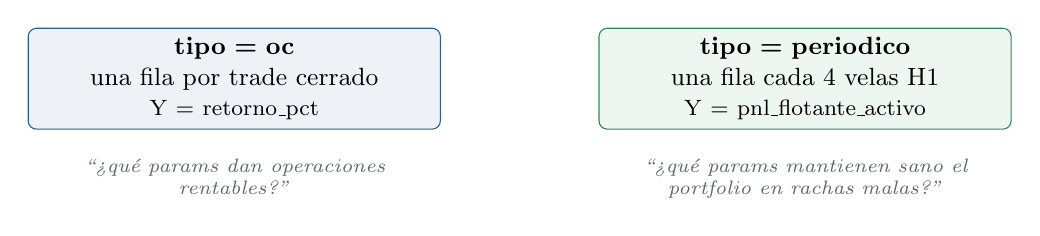
\begin{tikzpicture}[node distance=0.5cm]
  \node[caja, text width=5cm] (oc) {\textbf{tipo = oc}\\una fila por trade cerrado\\\footnotesize Y = retorno\_pct};
  \node[cajav, text width=5cm, right=2cm of oc] (per) {\textbf{tipo = periodico}\\una fila cada 4 velas H1\\\footnotesize Y = pnl\_flotante\_activo};
  \node[below=0.25cm of oc, text width=5cm, align=center, font=\scriptsize\itshape, text=cgris]
    {``¿qué params dan operaciones\\rentables?''};
  \node[below=0.25cm of per, text width=5cm, align=center, font=\scriptsize\itshape, text=cgris]
    {``¿qué params mantienen sano el\\portfolio en rachas malas?''};
\end{tikzpicture}}

\section{Por qué son necesarios los dos tipos}

Si el cuaderno solo guardara filas al cerrar operaciones, habría un \textbf{hueco peligroso}
durante las caídas sostenidas. Veámoslo:

\begin{ejemplo}[Una racha bajista de 3 días]
\begin{center}\small
\begin{tabular}{@{}lll@{}}
\toprule
Momento & Precio BTC & Qué pasa \\
\midrule
Lunes 09:00 & \$95.000 & 8 posiciones abiertas, todo normal. \\
Lunes 15:00 & \$92.000 & Posiciones en rojo. Ninguna cierra aún. \\
Martes 10:00 & \$88.000 & Más rojo. Ninguna cierra. \\
Miércoles & \$83.000 & Recién ahora empiezan a cerrar por PERDIDA\_MAX. \\
\bottomrule
\end{tabular}
\end{center}
Si solo guardáramos filas al cerrar órdenes, durante \textbf{3 días de caída el modelo no recibe
ningún dato nuevo}. No se entera de que el portfolio estaba sangrando. Cuando llega la primera
OC del miércoles, el daño ya está hecho.
\end{ejemplo}

La solución son los \textbf{registros periódicos}: cada 4 velas H1 (configurable con
\code{X5\_FREQ\_REGISTRO\_PERIODICO}), aunque no cierre ninguna orden, se guarda una fila con el
estado actual. Su variable objetivo es \code{pnl\_flotante\_activo}, que se vuelve cada vez más
negativo durante la caída. Así el modelo aprende: ``cuando el RSI cae bajo 30 y el drawdown supera
$-8\%$ con estos params, el portfolio se sigue deteriorando'' $\Rightarrow$ conviene reducir
exposición \emph{antes}.

\begin{nota}[Solo si hay posiciones abiertas]
Un registro periódico solo se genera si el activo tiene posiciones abiertas. Si no hay nada
expuesto al mercado, no hay \code{pnl\_flotante\_activo} que observar y la fila se omite.
\end{nota}

\section{Schema real implementado}

Lo que \code{X4\_backtester.py -{}-x5} escribe hoy en cada fila (puede diferir del diseño
aspiracional más ambicioso):

\begin{itemize}[itemsep=1pt, leftmargin=1.4em]
  \item \textbf{Identificadores}: \code{tipo\_registro}, \code{activo}, \code{timestamp\_oe},
  \code{timestamp\_oa}, \code{timestamp\_oc}.
  \item \textbf{Config activa (OE)}: \code{n\_ejecucion}, \code{K}, \code{N\_EXP}, \code{LAMBDA},
  \code{A}, \code{B}, \code{LOTAJES\_M}, \code{PERDIDA\_MAX}.
  \item \textbf{Temporales, X2, X3 (OE)} y sus versiones \textbf{(OA)} con sufijo \code{\_oa}.
  \item \textbf{Portfolio}: \code{n\_ordenes\_abiertas}, \code{n\_ordenes\_espera},
  \code{exposicion\_usd}, \code{mean\_retorno\_pct\_abierto}, \code{std\_retorno\_pct\_abierto},
  \code{retorno\_promedio\_ultimas\_5\_oc}, \code{pnl\_flotante\_activo}.
  \item \textbf{Targets}: \code{pnl\_cerrado\_activo}, \code{retorno\_pct}.
\end{itemize}

\begin{nota}[Acumulación sin truncar]
El store acumula \textbf{todas} las vueltas del backtesting, incluso las de configuraciones
malas. Los registros con params peores son igual de valiosos: le enseñan al modelo qué
\emph{no} funciona en cada régimen. Más variedad de (contexto, params, resultado) = más
relaciones causa-efecto que el modelo puede aprender.
\end{nota}

% ══════════════════════════════════════════════════════════════════════
\chapter{Arquitectura que escala con los datos}

\section{Tres niveles según cuántos datos hay}

X5 no arranca con una arquitectura fija. \textbf{Sube de nivel automáticamente} según cuántas
operaciones cerradas (OC) tenga el store de cada activo:

\diag{
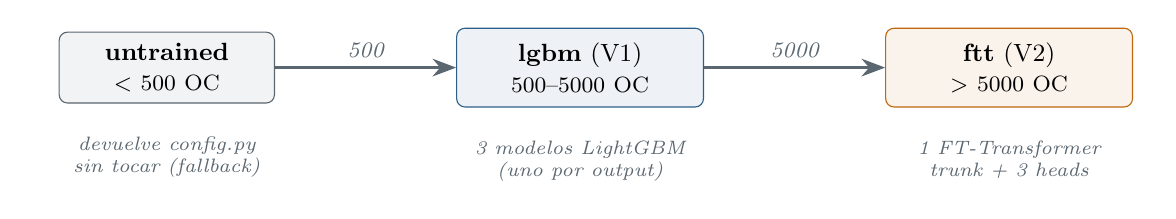
\begin{tikzpicture}[node distance=2.3cm]
  \node[cajag] (u) {\textbf{untrained}\\\footnotesize $<$ 500 OC};
  \node[caja, right=of u] (l) {\textbf{lgbm} (V1)\\\footnotesize 500--5000 OC};
  \node[cajan, right=of l] (f) {\textbf{ftt} (V2)\\\footnotesize $>$ 5000 OC};
  \draw[flecha] (u) -- (l) node[midway,above,etq]{500};
  \draw[flecha] (l) -- (f) node[midway,above,etq]{5000};
  \node[below=0.3cm of u, text width=3.3cm, align=center, font=\scriptsize\itshape, text=cgris]
    {devuelve config.py\\sin tocar (fallback)};
  \node[below=0.3cm of l, text width=3.3cm, align=center, font=\scriptsize\itshape, text=cgris]
    {3 modelos LightGBM\\(uno por output)};
  \node[below=0.3cm of f, text width=3.3cm, align=center, font=\scriptsize\itshape, text=cgris]
    {1 FT-Transformer\\trunk + 3 heads};
\end{tikzpicture}}

Los umbrales están en \code{config.py} (\code{X5\_MIN\_TRADES\_TRAIN=500},
\code{X5\_MIN\_TRADES\_FTT=5000}). La transición es \textbf{automática y por activo}: BTCUSD
puede estar en \code{ftt} mientras TSLA sigue en \code{untrained}, dentro de la misma corrida.

\begin{idea}[Por qué escalar y no empezar directo con la red grande]
Un FT-Transformer con pocos datos \emph{sobreajusta} (memoriza en vez de aprender). LightGBM
funciona muy bien con datasets pequeños. Empezar simple y crecer con los datos es más robusto
que arrancar con la arquitectura más potente y esperar a que ``cuaje''.
\end{idea}

\section{Estado actual}

El store está \textbf{vacío}: los 6 activos están en \code{untrained}. Mientras un activo esté
así, X5 devuelve los parámetros de \code{config.py} sin modificarlos (un \emph{fallback} seguro:
nunca deja que un modelo vacío rompa parámetros que funcionan). El objetivo de la Fase 1 es
recolectar datos para pasar a \code{lgbm}.

% ══════════════════════════════════════════════════════════════════════
\chapter{V1 — Gradient Boosting (LightGBM)}

\section{La intuición: un comité que corrige errores}

\textbf{Gradient Boosting} entrena muchos árboles de decisión \emph{en secuencia}, donde cada
árbol corrige los errores del anterior. No es una red neuronal. Es el punto de partida más
robusto para datos tabulares con pocas filas.

\begin{ejemplo}[Ejemplo numérico completo]
Queremos predecir el retorno de una operación. Tenemos 4 operaciones:
\begin{center}\small
\begin{tabular}{@{}lllll@{}}
\toprule
Op & RSI & K & Mercado & Retorno real \\
\midrule
A & 30 & 1.0 & bajista & $+3\%$ \\
B & 75 & 1.0 & alcista & $+1\%$ \\
C & 30 & 0.7 & bajista & $+4\%$ \\
D & 75 & 1.5 & alcista & $-1\%$ \\
\bottomrule
\end{tabular}
\end{center}

\textbf{Ronda 0 — predicción inicial.} Predice el promedio de todos: $(3+1+4-1)/4 = +1{,}75\%$
para todos. Los errores (real $-$ predicho) son:
\[
e_A = +1{,}25,\quad e_B = -0{,}75,\quad e_C = +2{,}25,\quad e_D = -2{,}75
\]

\textbf{Ronda 1 — primer árbol.} En vez de predecir el retorno, este árbol aprende a predecir los
\emph{errores}. Puede descubrir reglas simples como:
\begin{center}\small\ttfamily
si RSI $<$ 50 $\rightarrow$ corregir $+1.5\%$ \qquad si RSI $\geq$ 50 y K $>$ 1.2 $\rightarrow$ corregir $-2\%$
\end{center}
Aplicando estas correcciones, A sube a $+3{,}25\%$ y D baja a $-0{,}25\%$: nos acercamos.

\textbf{Ronda 2 — segundo árbol.} Aprende los errores que \emph{aún quedan}. Puede descubrir:
``si K $<$ 0.8 $\rightarrow$ corregir un poco más hacia arriba''.

\textbf{Y así 500 veces.} La predicción final es la suma:
\[
\text{retorno\_predicho} = \underbrace{1{,}75}_{\text{promedio}} + \text{corr}_1 + \text{corr}_2 + \cdots + \text{corr}_{500}
\]
\end{ejemplo}

Cada árbol es simple. La potencia viene de \textbf{acumular cientos de correcciones pequeñas y
específicas}. El término ``gradient'' viene de que las correcciones se calculan usando el gradiente
del error, lo que garantiza que cada árbol apunta en la dirección óptima de mejora.

\section{Cómo se ve en el código}

En X5, cuando un activo está en \code{lgbm}, se entrenan \textbf{3 modelos LightGBM independientes}
(uno por cada variable objetivo): \code{retorno}, \code{flotante}, \code{cerrado}. Cada uno es un
\code{LGBMRegressor} con \textasciitilde1000 árboles, \emph{early stopping} sobre un set de
validación, y regularización (\code{reg\_alpha}, \code{reg\_lambda}).

\begin{nota}[Un detalle importante del pipeline]
El modelo \code{flotante} (target \code{pnl\_flotante\_activo}) entrena con filas \code{oc}
\textbf{y} \code{periodico}, porque ese target existe en ambos tipos. Los modelos \code{retorno}
y \code{cerrado} entrenan solo con filas \code{oc}. Así los registros periódicos —diseñados para
capturar el deterioro en rachas malas— sí alimentan al modelo que más los necesita.
\end{nota}

\section{Ventajas y el único contra}

\begin{center}\small
\begin{tabular}{@{}p{7.5cm}p{7.5cm}@{}}
\toprule
\textbf{Ventajas} & \textbf{Contra} \\
\midrule
Funciona muy bien con $<$50k filas. No requiere normalización. Es interpretable (se ve qué
features importaron). Rápido de entrenar. &
\textbf{No es diferenciable} $\Rightarrow$ no se puede usar gradient ascent para la inferencia;
hay que usar Optuna (Capítulo 9), que es más lento. \\
\bottomrule
\end{tabular}
\end{center}

% ══════════════════════════════════════════════════════════════════════
\chapter{V2 — FT-Transformer (Feature Tokenizer + Transformer)}

Cuando el store supera \textasciitilde5000 OC, el salto natural es el \textbf{FT-Transformer}. Aquí
está el corazón conceptual del documento, así que iremos despacio.

\section{Paso 1 — Feature Tokenizer: cada número se vuelve un vector}

En una red neuronal común (un Perceptrón Multicapa, MLP), cada feature entra como un número
suelto. El modelo trata todos los números igual, sin saber que ``RSI'' y ``K'' son cosas
conceptualmente distintas.

El \textbf{Feature Tokenizer} convierte cada feature en un \textbf{vector} (embedding) propio:
\[
\text{embedding}_i = \text{valor}_i \times W_i + b_i
\]
donde $W_i$ y $b_i$ son un vector de pesos y un vector de sesgo, \emph{propios de esa feature y
aprendidos durante el entrenamiento}.

\begin{ejemplo}[Con D = 3 (en la práctica D = 192)]
\begin{align*}
\text{RSI} &= 72{,}3, \quad W_{RSI}=[0{,}5,\,-0{,}2,\,0{,}8], \quad b_{RSI}=[0{,}1,\,0{,}3,\,-0{,}1] \\
\text{embedding}_{RSI} &= 72{,}3 \times [0{,}5,\,-0{,}2,\,0{,}8] + [0{,}1,\,0{,}3,\,-0{,}1] \\
&= [36{,}15,\,-14{,}46,\,57{,}84] + [0{,}1,\,0{,}3,\,-0{,}1] = [36{,}25,\,-14{,}16,\,57{,}74]
\end{align*}
La feature \code{K} tiene \emph{sus propios} $W_K, b_K$, distintos. El modelo descubre por sí solo
qué transformación es útil para cada feature.
\end{ejemplo}

\diag{
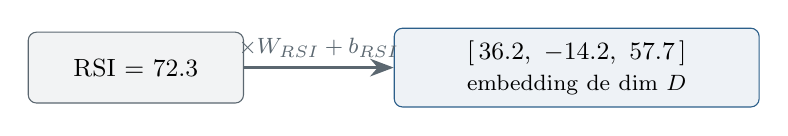
\begin{tikzpicture}[node distance=1.9cm]
  \node[cajag] (rsi) {RSI = 72.3};
  \node[caja, right=of rsi, text width=4.4cm] (emb) {$[\,36.2,\ -14.2,\ 57.7\,]$\\\footnotesize embedding de dim $D$};
  \draw[flecha] (rsi) -- (emb) node[midway,above,etq]{$\times W_{RSI}+b_{RSI}$};
\end{tikzpicture}}

La clave: comparado con una MLP donde RSI entra como el número ``72.3'', el FT-Transformer ve un
\textbf{vector de $D$ números que captura ``qué implica que RSI esté en este nivel''} según lo
aprendido. RSI=72 ``significa'' algo distinto que RSI=30, y esa diferencia queda representada.

\section{Paso 2 — Atención: las features se hablan entre sí}

\subsection{El problema que resuelve la atención}

Una MLP aprende la importancia de cada feature \emph{por separado}. Puede aprender ``RSI alto es
mala señal'', pero no ``RSI alto es mala señal \emph{solo cuando} la volatilidad también es alta
\emph{y} K $>$ 1.2''. Eso requiere capturar la interacción de tres features a la vez. La
\textbf{atención} hace exactamente eso: deja que cada feature ajuste su representación según el
contexto de todas las demás.

\subsection{La analogía de la reunión de equipo}

Imagina un equipo de 5 personas en una reunión. Cada persona es una feature:

\begin{center}\small
RSI: ``el precio está sobrecomprado (78)'' \quad\textbullet\quad K: ``el peso futuro es 1.5''\\
Volatilidad: ``el mercado está agitado'' \quad\textbullet\quad n\_sizes: ``hay 90 soportes''\\
Score fundamental: ``el activo está sano''
\end{center}

En una MLP, cada persona escribe su conclusión en un papel y la manda a la salida:
\textbf{no se hablan entre sí}. En un Transformer, \textbf{antes de concluir, cada persona
escucha a las demás y ajusta lo que va a decir}. RSI piensa: ``soy alto, normalmente mala
señal\ldots pero oí que la volatilidad también es alta y el fundamental es sano; en ese contexto
quizás no sea tan malo'', y ajusta su representación.

\subsection{El mecanismo concreto: Query, Key, Value}

Para que una feature pueda ``preguntar'' a las demás, el Transformer le asigna tres vectores,
derivados de su embedding con matrices aprendidas $W_Q, W_K, W_V$ (compartidas por todas):
\[
\begin{aligned}
Q_i &= \text{emb}_i\, W_Q \quad(\text{``qué busco''}) \\
K_i &= \text{emb}_i\, W_K \quad(\text{``qué ofrezco''}) \\
V_i &= \text{emb}_i\, W_V \quad(\text{``lo que comparto''})
\end{aligned}
\]

\begin{ejemplo}[RSI le pregunta a las demás]
RSI usa su $Q_{RSI}$ y mide su afinidad con cada compañera vía producto interno con los $K$:
\begin{center}\small
$Q_{RSI}\cdot K_{\text{Vol}} = 8{,}3$ \quad $Q_{RSI}\cdot K_{K} = 5{,}1$ \quad
$Q_{RSI}\cdot K_{\text{n\_sizes}} = 2{,}2$ \quad $Q_{RSI}\cdot K_{\text{fund}} = 4{,}7$
\end{center}
Aplica \textbf{softmax} para convertir esos scores en pesos que suman 1:
\[
\text{softmax}([8{,}3,\,5{,}1,\,2{,}2,\,4{,}7]) = [0{,}47,\ 0{,}22,\ 0{,}05,\ 0{,}26]
\]
El nuevo embedding de RSI es la suma ponderada de los \emph{Values}:
\[
\text{emb}_{RSI}^{\text{nuevo}} = 0{,}47\,V_{\text{Vol}} + 0{,}22\,V_{K} + 0{,}05\,V_{\text{n\_sizes}} + 0{,}26\,V_{\text{fund}}
\]
RSI ``absorbió'' información de las demás en proporción a cuánto le importaban. Su embedding ya
no es ``soy RSI = 78''; es ``soy RSI = 78 en un contexto de alta volatilidad, fundamental sano y
K = 1.5''.
\end{ejemplo}

\diag{
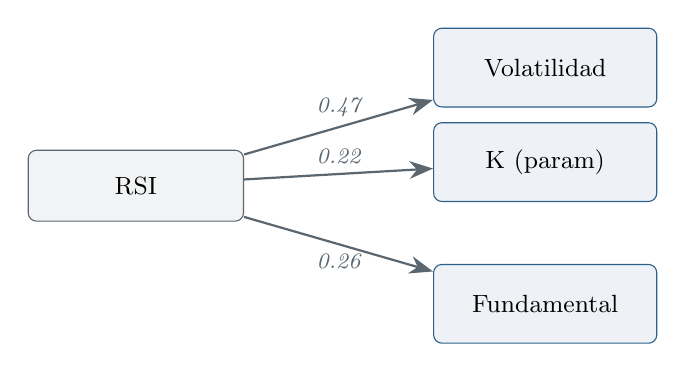
\begin{tikzpicture}[node distance=0.7cm and 2.4cm]
  \node[cajag] (rsi) {RSI};
  \node[caja, right=of rsi, yshift=1.5cm, text width=2.6cm] (vol) {Volatilidad};
  \node[caja, right=of rsi, yshift=0.3cm, text width=2.6cm] (k) {K (param)};
  \node[caja, right=of rsi, yshift=-1.5cm, text width=2.6cm] (fund) {Fundamental};
  \draw[flecha] (rsi) -- (vol) node[midway,above,etq]{0.47};
  \draw[flecha] (rsi) -- (k)   node[midway,above,etq]{0.22};
  \draw[flecha] (rsi) -- (fund) node[midway,below,etq]{0.26};
\end{tikzpicture}}

Esto ocurre \textbf{simultáneamente para todas las features}: cada una actualiza su representación
mirando a las demás.

\subsection{Multi-head: mirar desde varios ángulos}

Con una sola ``cabeza'' de atención, cada feature solo puede mirar a las demás desde un ángulo.
La \textbf{atención multi-cabeza} (Multi-Head Attention) corre el mecanismo varias veces en
paralelo, con matrices $W_Q, W_K, W_V$ distintas por cabeza:

\begin{center}\small
Cabeza 1: relaciones técnicas (RSI $\leftrightarrow$ Volatilidad $\leftrightarrow$ MACD)\\
Cabeza 2: relaciones params--contexto (K $\leftrightarrow$ tendencia $\leftrightarrow$ n\_sizes)\\
Cabeza 3: relaciones de riesgo (LOTAJES\_M $\leftrightarrow$ exposición $\leftrightarrow$ drawdown)
\end{center}

Los resultados de todas las cabezas se concatenan y se proyectan en un vector final. Así el modelo
captura múltiples tipos de relación a la vez, sin que una interfiera con otra.

\section{Paso 3 — Apilar capas: de lo simple a lo abstracto}

Un solo bloque de atención captura relaciones directas. Pero algunos patrones son más abstractos:
``el efecto de K depende de la volatilidad, que a su vez depende del régimen, que se infiere
combinando score + MACD + tendencia''. Por eso el Transformer apila varias capas:

\diag{
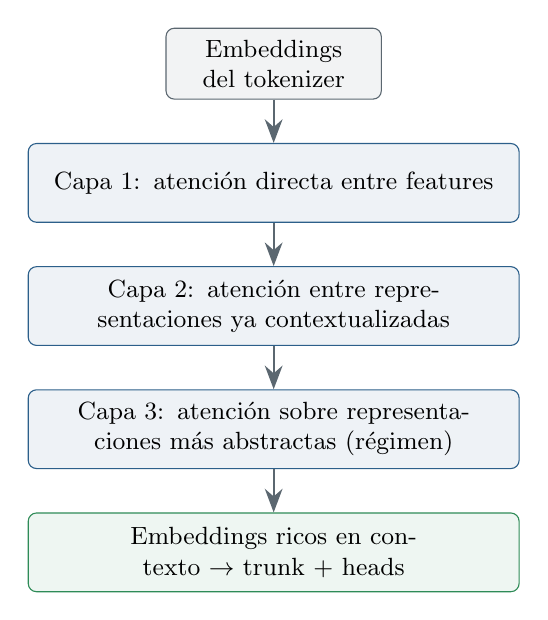
\begin{tikzpicture}[node distance=0.55cm]
  \node[cajag] (in) {Embeddings del tokenizer};
  \node[caja, below=of in, text width=6cm] (c1) {Capa 1: atención directa entre features};
  \node[caja, below=of c1, text width=6cm] (c2) {Capa 2: atención entre representaciones ya contextualizadas};
  \node[caja, below=of c2, text width=6cm] (c3) {Capa 3: atención sobre representaciones más abstractas (régimen)};
  \node[cajav, below=of c3, text width=6cm] (out) {Embeddings ricos en contexto $\rightarrow$ trunk + heads};
  \draw[flecha] (in) -- (c1);
  \draw[flecha] (c1) -- (c2);
  \draw[flecha] (c2) -- (c3);
  \draw[flecha] (c3) -- (out);
\end{tikzpicture}}

Para datos tabulares como los de X5, \textbf{2--4 capas} suelen bastar. (Los grandes modelos de
lenguaje usan 32--96 capas porque el lenguaje es mucho más complejo.)

\section{Dentro de cada bloque Transformer}

Cada capa no es solo atención pura. El bloque completo (variante \emph{pre-norm}, más estable)
es: normalización $\rightarrow$ atención $\rightarrow$ conexión residual $\rightarrow$
normalización $\rightarrow$ MLP $\rightarrow$ conexión residual.

\begin{center}
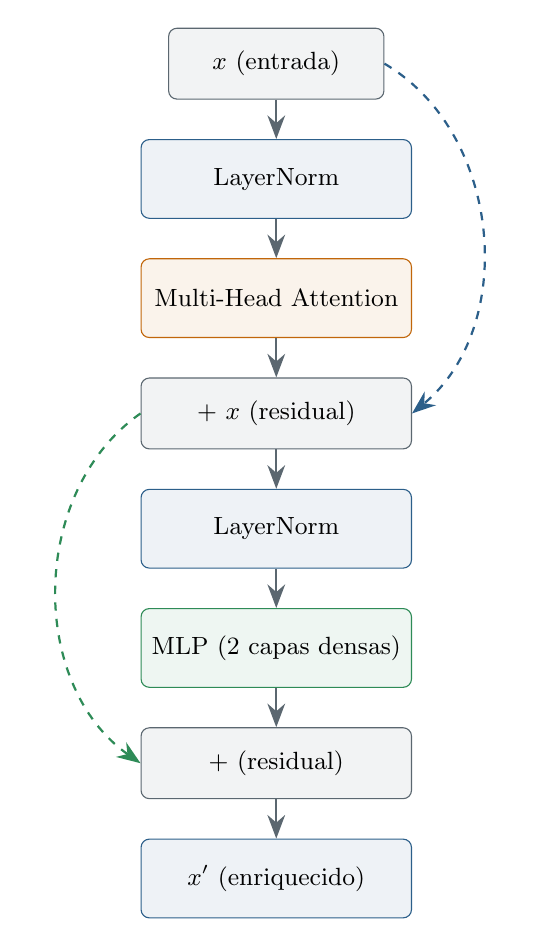
\begin{tikzpicture}[node distance=0.5cm]
  \node[cajag] (x) {$x$ (entrada)};
  \node[caja, below=of x, text width=3.2cm] (n1) {LayerNorm};
  \node[cajan, below=of n1, text width=3.2cm] (mha) {Multi-Head Attention};
  \node[cajag, below=of mha, text width=3.2cm] (s1) {$+\ x$ (residual)};
  \node[caja, below=of s1, text width=3.2cm] (n2) {LayerNorm};
  \node[cajav, below=of n2, text width=3.2cm] (ffn) {MLP (2 capas densas)};
  \node[cajag, below=of ffn, text width=3.2cm] (s2) {$+$ (residual)};
  \node[caja, below=of s2, text width=3.2cm] (out) {$x'$ (enriquecido)};
  \draw[flecha] (x)--(n1); \draw[flecha] (n1)--(mha); \draw[flecha] (mha)--(s1);
  \draw[flecha] (s1)--(n2); \draw[flecha] (n2)--(ffn); \draw[flecha] (ffn)--(s2); \draw[flecha] (s2)--(out);
  \draw[flecha, dashed, draw=cazul] (x.east) to[bend left=55] (s1.east);
  \draw[flecha, dashed, draw=cverde] (s1.west) to[bend right=55] (s2.west);
\end{tikzpicture}
\end{center}

\begin{itemize}[leftmargin=1.4em]
  \item \textbf{Conexión residual} (líneas punteadas): se suma la entrada de la capa a su salida.
  Garantiza que si la capa no aporta nada útil, puede aprender a devolver el input intacto, y el
  gradiente fluye sin degradarse. Sin esto, apilar más de 2--3 capas es muy difícil de entrenar.
  \item \textbf{LayerNorm}: normaliza el embedding (media 0, desviación 1) antes de cada
  sub-bloque. Estabiliza el entrenamiento.
  \item \textbf{MLP interno}: tras absorber contexto, cada feature pasa por un pequeño perceptrón
  que transforma su representación de formas más complejas que la atención sola.
\end{itemize}

\section{La salida multi-head: predecir 3 cosas a la vez}

Tras las capas Transformer, un \textbf{trunk} (tronco) compartido produce una representación
general, y tres \textbf{heads} (cabezas) predicen cada variable objetivo:

\diag{
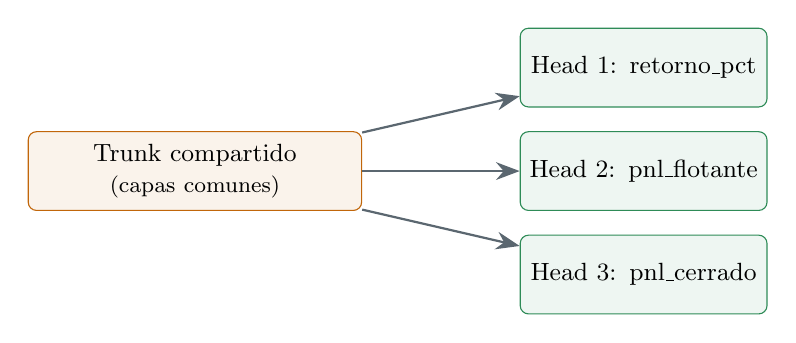
\begin{tikzpicture}[node distance=1.1cm]
  \node[cajan, text width=4cm] (trunk) {Trunk compartido\\\footnotesize (capas comunes)};
  \node[cajav, above right=0.3cm and 2cm of trunk] (h1) {Head 1: retorno\_pct};
  \node[cajav, right=2cm of trunk] (h2) {Head 2: pnl\_flotante};
  \node[cajav, below right=0.3cm and 2cm of trunk] (h3) {Head 3: pnl\_cerrado};
  \draw[flecha] (trunk)--(h1); \draw[flecha] (trunk)--(h2); \draw[flecha] (trunk)--(h3);
\end{tikzpicture}}

\begin{idea}[Por qué multi-head es mejor que 3 modelos separados]
Como un médico que hace una sola revisión (el trunk) y luego da tres diagnósticos
(cardiovascular, respiratorio, metabólico). Compartir el trunk actúa como \textbf{regularización}:
el modelo no puede sobreajustarse a una señal ruidosa individual si tiene que explicar tres
variables a la vez con la misma representación base.
\end{idea}

\begin{nota}[Estado real vs.\ diseño]
En LightGBM las 3 salidas son 3 modelos independientes. La arquitectura multi-head aplica en
V2 (FTT). Hoy, en FTT, los 3 heads comparten el tensor de filas \code{oc}; incorporar las filas
periódicas al head flotante en FTT (como sí ocurre en LightGBM) es un TO DO pendiente.
\end{nota}

% ══════════════════════════════════════════════════════════════════════
\chapter{Inferencia: encontrar los parámetros óptimos}

Con el contexto de mercado de hoy \textbf{fijo}, queremos los params que maximizan el retorno
predicho. La estrategia depende del tipo de modelo.

\section{Con LightGBM: búsqueda con Optuna}

LightGBM no es diferenciable, así que no podemos hacer matemática continua sobre él. La estrategia:

\begin{enumerate}[leftmargin=1.5em, itemsep=1pt]
  \item Fijar el contexto de mercado actual (X2 + X3).
  \item Probar muchas combinaciones de parámetros.
  \item Para cada una, preguntarle al modelo: ``¿cuánto predices que gano con estos params?''.
  \item Quedarse con la combinación de mayor predicción.
\end{enumerate}

En vez de una rejilla ciega, se usa \textbf{Optuna}, un optimizador \emph{bayesiano}: aprende qué
zonas del espacio de parámetros son prometedoras y concentra ahí los intentos, en vez de probar
todo por igual. Por defecto \textbf{200 trials} (\code{X5\_N\_OPTUNA\_TRIALS}). Es como pedirle al
comité de expertos que evalúe 200 recetas y elija la mejor para la cocina de hoy.

\section{Con FT-Transformer: gradient ascent}

Una red neuronal es una función matemática \textbf{diferenciable}. Podemos calcular: ``si subo K
en 0.01, ¿el retorno predicho sube o baja, y cuánto?''. El \textbf{gradient ascent} aprovecha eso:

\begin{enumerate}[leftmargin=1.5em, itemsep=1pt]
  \item Fijar el contexto (no se toca).
  \item Inicializar los params en algún punto del espacio.
  \item Calcular el gradiente respecto a los \emph{params de entrada} (no a los pesos del modelo).
  \item Dar un paso en la dirección que sube el retorno.
  \item Repetir hasta llegar a un máximo.
\end{enumerate}

\diag{
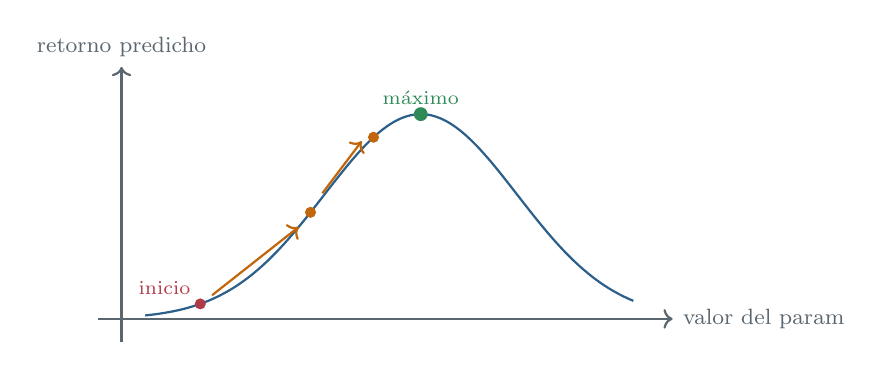
\begin{tikzpicture}[scale=1]
  \draw[->, thick, cgris] (-0.3,0) -- (7,0) node[right,font=\footnotesize] {valor del param};
  \draw[->, thick, cgris] (0,-0.3) -- (0,3.2) node[above,font=\footnotesize] {retorno predicho};
  \draw[thick, cazul, domain=0.3:6.5, samples=100] plot (\x, {2.6*exp(-(\x-3.8)^2/3)});
  \fill[crojo] (1,{2.6*exp(-(1-3.8)^2/3)}) circle (2pt) node[above left,font=\scriptsize]{inicio};
  \fill[cnaranja] (2.4,{2.6*exp(-(2.4-3.8)^2/3)}) circle (2pt);
  \fill[cnaranja] (3.2,{2.6*exp(-(3.2-3.8)^2/3)}) circle (2pt);
  \fill[cverde] (3.8,2.6) circle (2.5pt) node[above,font=\scriptsize]{máximo};
  \draw[->,cnaranja,thick] (1.15,{2.6*exp(-(1.15-3.8)^2/3)+0.05}) -- (2.25,{2.6*exp(-(2.25-3.8)^2/3)});
  \draw[->,cnaranja,thick] (2.55,{2.6*exp(-(2.55-3.8)^2/3)+0.05}) -- (3.05,{2.6*exp(-(3.05-3.8)^2/3)+0.1});
\end{tikzpicture}}

\begin{idea}[La analogía de la colina con los ojos vendados]
Estás en una colina y quieres llegar a la cima, pero con los ojos vendados. En cada paso tocas
el suelo con el pie para sentir hacia dónde sube la pendiente y avanzas en esa dirección. El
gradient ascent es eso, pero matemático. Es mucho más eficiente que probar 200 combinaciones a
ciegas. El contra: puede quedar atrapado en una colina pequeña (máximo local); se mitiga
repitiendo desde varios puntos de inicio aleatorios (\code{X5\_ASCENT\_RESTARTS}).
\end{idea}

Al final, los params se \textbf{redondean} (los enteros como \code{LOTAJES\_M}) y se
\textbf{recortan} a sus rangos válidos.

% ══════════════════════════════════════════════════════════════════════
\chapter{El airbag: la red de seguridad dura}

El modelo aprende patrones del pasado. Un crash repentino puede ser tan distinto a todo lo que
vio que \textbf{no reaccione a tiempo}: recomienda params normales mientras el precio cae 8\% en
4 horas. Para ese caso existe el \textbf{airbag}: una regla \emph{explícita, no aprendida}, que
actúa independientemente de lo que el modelo recomiende.

\begin{center}\small\ttfamily
Si en las últimas 4 velas H1 el precio cayó más del umbral:\\
$\rightarrow$ forzar LOTAJES\_M al mínimo (1)\\
$\rightarrow$ forzar n\_sizes\_ejecucion al mínimo permitido
\end{center}

Los umbrales van en \code{config.py}: \textbf{8\% para crypto, 5\% para acciones}
(\code{X5\_AIRBAG\_THRESHOLD}).

\begin{nota}[El airbag es el último recurso, no el mecanismo principal]
La idea es que, con suficiente historia de crashes, el modelo aprenda a recomendar params
conservadores \emph{antes} de que el airbag se active. Si el airbag se dispara muy seguido, es
señal de que el modelo necesita más datos de ese tipo de escenario. El airbag cubre el riesgo de
mercado; el estado \code{untrained} cubre el riesgo de que el modelo aún no sepa.
\end{nota}

% ══════════════════════════════════════════════════════════════════════
\chapter{El sesgo de selección y la exploración}

\section{El problema más sutil (y más importante)}

El cuaderno solo contiene operaciones hechas con los params que el sistema consideraba ``buenos''
en ese momento. \textbf{Nunca vemos qué habría pasado con otros params}, porque nunca los
probamos.

\begin{idea}[La analogía del restaurante]
Quieres saber cuál es el mejor restaurante de la ciudad. Pero siempre vas al mismo porque te
parece bueno. Al final del año tienes 200 reseñas de ese restaurante y cero del resto. No puedes
concluir que es el mejor: nunca probaste los otros. El modelo cae en la misma trampa: aprende
que ``los params actuales son buenos'' simplemente porque son los únicos que vio.
\end{idea}

\section{La solución: exploración deliberada por ciclo completo}

En el backtesting, una fracción de los ciclos usa params \textbf{aleatorios} (exploración) en
vez del mejor conocido (explotación):

\diag{

\begin{tikzpicture}[node distance=0.35cm]
  \node[cajav] (c1) {Ciclo 1\\EXPLOIT};
  \node[cajan, right=of c1] (c2) {Ciclo 2\\EXPLORE};
  \node[cajav, right=of c2] (c3) {Ciclo 3\\EXPLOIT};
  \node[cajan, right=of c3] (c4) {Ciclo 4\\EXPLORE};
  \node[cajav, right=of c4] (c5) {Ciclo 5\\EXPLOIT};
  \node[cajag, right=of c5] (cn) {\ldots};
  \draw[flecha] (c1)--(c2); \draw[flecha] (c2)--(c3); \draw[flecha] (c3)--(c4);
  \draw[flecha] (c4)--(c5); \draw[flecha] (c5)--(cn);
\end{tikzpicture}}

Un $\sim$30\% de exploración (\code{X5\_EXPLORATION\_RATE}) es un punto de partida razonable.

\begin{nota}[Por qué por ciclo entero y no vela a vela]
El backtesting recorre \textasciitilde2 años de historia por ciclo (con mercados alcistas,
bajistas, laterales, crashes). Si aleatorizamos los params \emph{al inicio del ciclo} y los
mantenemos fijos, el modelo ve ``cómo funcionaron ESTOS params en TODO tipo de mercado''. Puede
aprender que K=1.5 va bien en bull pero falla en crashes, porque ambos escenarios están en el
mismo ciclo. Si aleatorizáramos vela a vela, habría demasiado ruido para atribuir el resultado
al contexto.
\end{nota}

Los ciclos EXPLORE rinden peor a propósito. Eso \textbf{no importa}: su objetivo no es ganar,
sino generar datos variados. Son los ciclos más valiosos para que el modelo aprenda qué
\emph{no} funciona en cada régimen.

% ══════════════════════════════════════════════════════════════════════
\chapter{No-estacionariedad, overfitting y portfolio}

\section{No-estacionariedad: el mercado cambia de personalidad}

Un modelo entrenado en el bull market de 2024 puede ser inútil en el bear market de 2026: los
patrones que aprendió ya no aplican. Esto se llama \textbf{concept drift}.

\textbf{Solución — ponderación temporal exponencial:} entrenar con todo el historial, pero dando
más peso a las operaciones recientes:
\[
\text{peso de una operación} = e^{-\lambda \cdot \text{días de antigüedad}}
\]
Con $\lambda$ alto, el modelo ``olvida'' rápido; con $\lambda$ bajo, valora más la historia. En
X5 esto es \code{X5\_LAMBDA\_DECAY} (por defecto 0.001, que da peso $\approx 0{,}5$ a operaciones
de \textasciitilde700 días atrás). Es una sola línea en el \code{sample\_weight} del entrenamiento
y no descarta datos valiosos del pasado.

\section{Overfitting: el estudiante que memoriza}

\textbf{Overfitting} = el modelo memoriza los datos de entrenamiento en vez de aprender patrones
generalizables. Como un estudiante que memoriza las respuestas exactas de exámenes pasados: saca
100 en ésos, pero falla cuando cambian la redacción. Señales: error muy bajo en train pero alto
en datos nuevos; el modelo recomienda siempre los mismos params extremos.

\textbf{Cómo se mitiga:}
\begin{enumerate}[leftmargin=1.5em, itemsep=1pt]
  \item \textbf{Normalizar en \%, no en USD}: ganar \$500 en una cuenta grande no es lo mismo que
  en una chica; en \% la señal es comparable.
  \item \textbf{Dropout}: apagar aleatoriamente algunas neuronas en cada pasada (fuerza redundancia).
  \item \textbf{Regularización L2}: penaliza pesos muy grandes (evita depender de una sola feature).
  \item \textbf{Validación temporal}: siempre entrenar con el pasado y validar con el futuro
  (nunca al revés), para no ``filtrar'' información futura.
  \item \textbf{Multi-head}: predecir 3 variables a la vez obliga al trunk a aprender
  representaciones generales.
\end{enumerate}

\section{Representación del portfolio (Deep Sets)}

Al abrir una nueva orden, el activo puede tener $N$ posiciones abiertas, y $N$ varía (a veces 2, a
veces 8). Pero una red neuronal espera entradas de \textbf{tamaño fijo}. Hay dos soluciones:

\begin{itemize}[leftmargin=1.4em]
  \item \textbf{V1 — estadísticas resumidas} (la que se usa): en vez de las órdenes individuales,
  se pasan resúmenes: \code{n\_ordenes\_abiertas}, media y desviación del retorno flotante,
  exposición \%. Siempre son los mismos números, sin importar cuántas órdenes haya. Además evita
  que el modelo aprenda ``identidades'' espurias de órdenes concretas.
  \item \textbf{V2 — Deep Sets (mean pooling)}: cada orden se codifica como un vector pequeño
  $[\text{retorno flotante}, \text{horas abierta}, \text{distancia entrada}, \text{lote}]$, y se
  \emph{promedian} todos. El promedio es \textbf{permutation-invariant}: da igual el orden en que
  se listen las órdenes (el promedio de $[3,5,7]$ es el mismo que el de $[7,3,5]$). Así el modelo
  no aprende un sesgo artificial del tipo ``la orden \#1 siempre importa más''.
\end{itemize}

% ══════════════════════════════════════════════════════════════════════
\chapter{Métricas de performance del modelo}

Cada vez que X5 entrena, calcula y guarda métricas clásicas de Aprendizaje Automático en
\code{resources/x5/Performance/\{ACTIVO\}\_performance.json} (historial, con \emph{split} 80/20
cronológico, no aleatorio, para respetar el orden temporal). Para cada target y cada set
(train/test):

\begin{center}\small
\begin{tabular}{@{}llp{7.2cm}@{}}
\toprule
\textbf{Métrica} & \textbf{Fórmula} & \textbf{Qué mide} \\
\midrule
MAE & $\text{mean}(|y-\hat y|)$ & Error absoluto promedio, en las unidades del target. \\
MSE & $\text{mean}((y-\hat y)^2)$ & Penaliza los errores grandes cuadráticamente. \\
MAPE & $100\cdot\text{mean}(|y-\hat y|/|y|)$ & Error porcentual relativo. \code{None} si $|y|\approx 0$. \\
$R^2$ & $1 - \text{SS}_{\text{res}}/\text{SS}_{\text{tot}}$ & \% de varianza explicada. 1 = perfecto, 0 = predecir la media, negativo = peor que la media. \\
\bottomrule
\end{tabular}
\end{center}

\begin{nota}[Señales de alerta]
\begin{itemize}[itemsep=1pt, leftmargin=1.2em]
  \item $R^2_{\text{train}} \gg R^2_{\text{test}}$: overfitting claro.
  \item $R^2_{\text{test}} < 0$: el modelo es peor que predecir la media (store con mucho ruido o
  poca variedad de contextos).
  \item MAE test creciente entre entrenamientos: el modelo se está degradando.
  \item MAPE \code{None} frecuente en \code{flotante}/\code{cerrado}: normal (targets cercanos a 0);
  usar MAE y $R^2$ para esos heads.
\end{itemize}
La evolución de estas métricas es la fuente principal para decidir cuándo pasar de V1 a V2 y para
calibrar los umbrales.
\end{nota}

% ══════════════════════════════════════════════════════════════════════
\chapter{Las dos fases de rollout}

X5 se integra en dos fases. El interruptor es \code{TIPO\_EJECUCION} en \code{config.py}.

\diag{
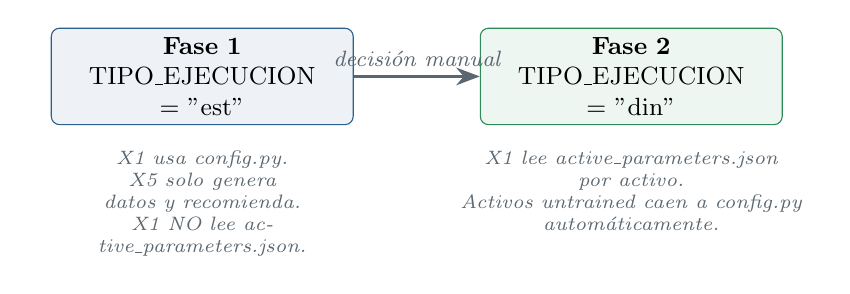
\begin{tikzpicture}[node distance=1.0cm and 1.6cm]
  \node[caja, text width=3.6cm] (est) {\textbf{Fase 1}\\TIPO\_EJECUCION = "est"};
  \node[cajav, right=of est, text width=3.6cm] (din) {\textbf{Fase 2}\\TIPO\_EJECUCION = "din"};
  \node[below=0.2cm of est, text width=4.2cm, align=center, font=\scriptsize\itshape, text=cgris]
    {X1 usa config.py.\\X5 solo genera datos y recomienda.\\X1 NO lee active\_parameters.json.};
  \node[below=0.2cm of din, text width=4.6cm, align=center, font=\scriptsize\itshape, text=cgris]
    {X1 lee active\_parameters.json por activo.\\Activos untrained caen a config.py\\automáticamente.};
  \draw[flecha] (est) -- (din) node[midway,above,etq]{decisión manual};
\end{tikzpicture}}

\begin{center}\small
\begin{tabular}{@{}lll@{}}
\toprule
\code{model\_status} & Significado & Qué usa X1 (en Fase 2) \\
\midrule
\code{untrained} & $<$500 OC, sin datos. & \code{config.py} (fallback). \\
\code{lgbm} & Modelo V1 activo. & params de \code{active\_parameters.json}. \\
\code{ftt} & Modelo V2 activo. & params de \code{active\_parameters.json}. \\
\bottomrule
\end{tabular}
\end{center}

La transición es \textbf{por activo}: BTCUSD puede estar en \code{din} usando su modelo mientras
TSLA sigue cayendo a \code{config.py}, todo en la misma corrida. Cambiar a Fase 2 es la única
acción manual, y se hace cuando las métricas dan confianza.

\begin{idea}[El ciclo de retroalimentación cerrado (objetivo final)]
En Fase 2, X1 opera con params dinámicos y genera trades reales, que alimentan el store, que
reentrena el modelo, que mejora los params que usa X1. El sistema se corrige solo. Los
backtesters dejan de ser la fuente principal de datos a medida que X1 en vivo acumula operaciones
reales con variedad de contextos.
\end{idea}

% ══════════════════════════════════════════════════════════════════════
\chapter{Cómo ejecutar X5 desde cero}

\section{El mapa mental}

\diag{
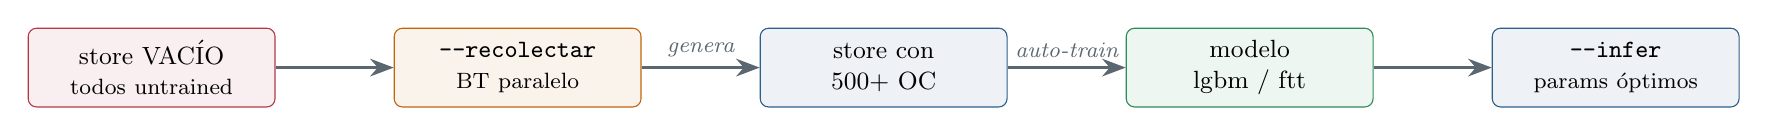
\begin{tikzpicture}[node distance=0.7cm and 1.5cm]
  \node[cajar] (v) {store VACÍO\\\footnotesize todos untrained};
  \node[cajan, right=of v] (r) {\code{-{}-recolectar}\\\footnotesize BT paralelo};
  \node[caja, right=of r] (d) {store con\\500+ OC};
  \node[cajav, right=of d] (m) {modelo\\lgbm / ftt};
  \node[caja, right=of m] (i) {\code{-{}-infer}\\\footnotesize params óptimos};
  \draw[flecha] (v)--(r); \draw[flecha] (r)--(d) node[midway,above,etq]{genera};
  \draw[flecha] (d)--(m) node[midway,above,etq]{auto-train}; \draw[flecha] (m)--(i);
\end{tikzpicture}}

\section{Los 3 modos (+ una casilla)}

X5 se simplificó de 5 modos a 3 + una casilla. \code{-{}-vela} fue eliminado (era un alias
exacto de \code{-{}-infer}).

\begin{lstlisting}[language=bash]
python scripts/X5_macro_brain.py --recolectar --version V1  # generar datos + entrenar
python scripts/X5_macro_brain.py --infer                    # recomendar params
python scripts/X5_macro_brain.py --infer --train            # reentrenar y recomendar
python scripts/X5_macro_brain.py --status                   # diagnostico
python scripts/X5_macro_brain.py --infer --activo BTCUSD    # solo un activo (merge)
\end{lstlisting}

\section{Paso a paso}

\textbf{Paso 0 — Requisitos.} Datos en \code{Data/} y \code{Data\_minuto/} (los genera X0),
scores en \code{resources/x2/}, y las dependencias \code{lightgbm}, \code{torch}, \code{optuna}.

\textbf{Paso 1 — Ver el estado.}
\begin{lstlisting}[language=bash]
python scripts/X5_macro_brain.py --status
\end{lstlisting}
Al inicio: 0 OC y \code{untrained} en los 6 activos. Es lo esperado.

\textbf{Paso 2 — Recolectar (el paso principal y más largo).}
\begin{lstlisting}[language=bash]
python scripts/X5_macro_brain.py --recolectar --version V1
\end{lstlisting}

Qué pasa por dentro:

\diag{
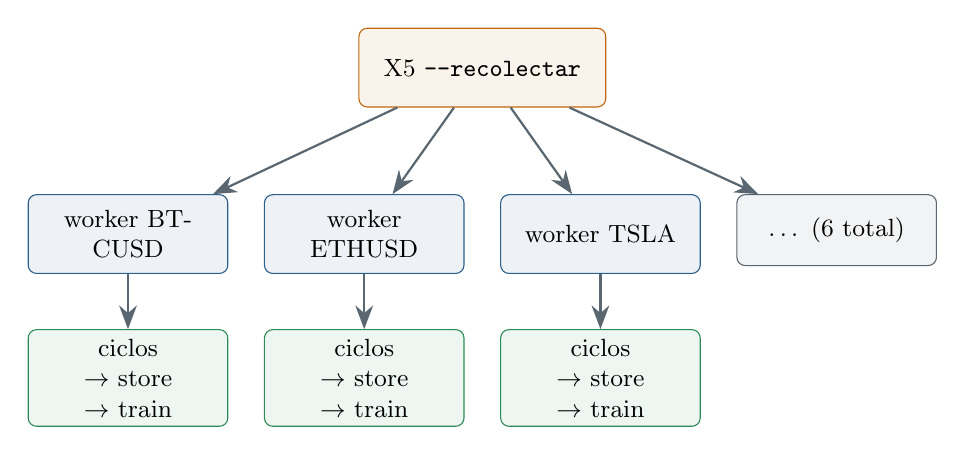
\begin{tikzpicture}[node distance=0.45cm and 0.9cm]
  \node[cajan] (x5) {X5 \code{-{}-recolectar}};
  \node[caja, below=1.1cm of x5, xshift=-4.5cm, text width=2.3cm] (w1) {worker BTCUSD};
  \node[caja, below=1.1cm of x5, xshift=-1.5cm, text width=2.3cm] (w2) {worker ETHUSD};
  \node[caja, below=1.1cm of x5, xshift=1.5cm, text width=2.3cm] (w3) {worker TSLA};
  \node[cajag, below=1.1cm of x5, xshift=4.5cm, text width=2.3cm] (wn) {\ldots\ (6 total)};
  \draw[flecha] (x5)--(w1); \draw[flecha] (x5)--(w2); \draw[flecha] (x5)--(w3); \draw[flecha] (x5)--(wn);
  \node[cajav, below=0.7cm of w1, text width=2.3cm] (s1) {ciclos\\$\rightarrow$ store\\$\rightarrow$ train};
  \node[cajav, below=0.7cm of w2, text width=2.3cm] (s2) {ciclos\\$\rightarrow$ store\\$\rightarrow$ train};
  \node[cajav, below=0.7cm of w3, text width=2.3cm] (s3) {ciclos\\$\rightarrow$ store\\$\rightarrow$ train};
  \draw[flecha] (w1)--(s1); \draw[flecha] (w2)--(s2); \draw[flecha] (w3)--(s3);
\end{tikzpicture}}

\begin{itemize}[leftmargin=1.4em, itemsep=1pt]
  \item X5 lanza \textbf{6 workers en paralelo}, uno por activo (como 6 chefs cocinando cada uno
  en su cocina).
  \item Cada worker corre un \textbf{ciclo} = un backtest completo desde \code{fecha\_inicio},
  simulando X1 vela a vela y anotando filas en su cuaderno.
  \item Al terminar el ciclo, \textbf{reinicia desde \code{fecha\_inicio}} con otros params
  (explore/exploit), y así hasta \code{X5\_N\_CICLOS\_BT} ciclos o \code{X5\_MIN\_TRADES\_FTT} OC.
  \item \textbf{Apenas un activo cruza 500 OC, ese worker entrena su modelo} sin esperar a los
  demás. Desde ahí sus ciclos EXPLOIT usan el modelo recién entrenado: \emph{los params se van
  corrigiendo por activo}.
  \item \textbf{Aislamiento}: cada worker usa su carpeta \code{resources\_\{V\}\_\{ACTIVO\}} para el
  checkpoint/equity de X4; el cuaderno ya es por activo. Así 6 procesos no se pisan.
\end{itemize}

\begin{nota}[El primer ciclo es lento]
El primer ciclo de cada activo hace \emph{cold start}: recalcula soportes desde cero (varios
minutos). Los ciclos siguientes reutilizan la cache de soportes de ese activo.
\end{nota}

\textbf{Paso 3 — Confirmar modelos.} Repetir \code{-{}-status}: deberías ver activos en
\code{lgbm} (500--5000 OC) o \code{ftt} ($>$5000). Las métricas quedan en
\code{resources/x5/Performance/}.

\textbf{Paso 4 — Recomendar params.}
\begin{lstlisting}[language=bash]
python scripts/X5_macro_brain.py --infer
\end{lstlisting}
Lee el contexto actual, busca los params que maximizan \code{retorno\_pct} y los escribe en
\code{config/active\_parameters.json}. Los activos aún \code{untrained} salen con sus valores de
\code{config.py}.

\textbf{Paso 5 — Activar Fase 2} (cuando confíes en las métricas): en \code{config.py} poner
\code{TIPO\_EJECUCION = "din"}.

\section{Preguntas frecuentes}

\begin{description}[leftmargin=0pt, itemsep=2pt]
  \item[\textmd{\textit{¿Tengo que llamar \code{-{}-train} aparte?}}] No. \code{-{}-recolectar} ya
  entrena solo cuando cada activo cruza el umbral. \code{-{}-train} es solo la casilla de
  \code{-{}-infer} para forzar un reentreno puntual.
  \item[\textmd{\textit{¿\code{-{}-recolectar} borra lo anterior?}}] No borra el cuaderno (acumula).
  Cada ciclo de backtest sí parte de cero en la simulación, pero las filas se \emph{agregan}.
  \item[\textmd{\textit{¿Puedo cortar y retomar?}}] Sí. El store persiste en disco; al relanzar,
  cada worker sigue sumando sobre lo que ya había.
  \item[\textmd{\textit{¿Por qué en paralelo?}}] Para que los 6 activos avancen a la vez y cada uno
  corrija sus params apenas tenga datos, en vez de esperar a que termine uno para empezar el otro.
\end{description}

% ══════════════════════════════════════════════════════════════════════
\chapter{Parámetros de configuración de X5}

Todos en \code{config.py}, bajo el bloque de X5:

\begin{center}\small
\begin{tabular}{@{}lll@{}}
\toprule
\textbf{Parámetro} & \textbf{Valor} & \textbf{Qué controla} \\
\midrule
\code{TIPO\_EJECUCION} & "est" & Fase 1 (est) o Fase 2 (din). \\
\code{X5\_EXPLORATION\_RATE} & 0.30 & Fracción de ciclos con params aleatorios. \\
\code{X5\_FREQ\_REGISTRO\_PERIODICO} & 4 & Snapshot periódico cada N velas H1. \\
\code{X5\_N\_CICLOS\_BT} & 20 & Máx.\ de ciclos por activo en \code{-{}-recolectar}. \\
\code{X5\_MIN\_TRADES\_TRAIN} & 500 & OC mínimas para entrenar (bajo esto: untrained). \\
\code{X5\_MIN\_TRADES\_FTT} & 5000 & OC para pasar de LightGBM a FT-Transformer. \\
\code{X5\_RETRAIN\_EVERY\_N\_VELAS} & 48 & Reentrenamiento completo (modo LightGBM). \\
\code{X5\_WINDOW\_TRAIN} & None & Ventana de entrenamiento (None = todo el store). \\
\code{X5\_LAMBDA\_DECAY} & 0.001 & Decaimiento del peso temporal. \\
\code{X5\_N\_OPTUNA\_TRIALS} & 200 & Intentos de Optuna por inferencia (LightGBM). \\
\code{X5\_ASCENT\_RESTARTS} & 10 & Puntos de inicio del gradient ascent (FTT). \\
\code{X5\_ASCENT\_STEPS} & 300 & Pasos de ascent por inicio. \\
\code{X5\_ASCENT\_LR} & 0.01 & Tamaño del paso del ascent. \\
\code{X5\_AIRBAG\_THRESHOLD} & 8\% / 5\% & Caída que dispara el airbag (crypto / acciones). \\
\code{X5\_N\_MINIMO} & 30 / 20 & N mínimo al activar el airbag. \\
\code{X5\_PARAM\_RANGES} & — & Rangos de búsqueda de cada param, por activo. \\
\bottomrule
\end{tabular}
\end{center}

% ══════════════════════════════════════════════════════════════════════
\chapter{Glosario completo}

\begin{description}[leftmargin=0pt, itemsep=2.5pt]
  \item[\textmd{\textbf{Surrogate model}}] Modelo que imita el sistema real para predecir barato el resultado de una operación.
  \item[\textmd{\textbf{Tabular data}}] Datos en filas y columnas (como Excel). Cada fila una operación, cada columna una feature.
  \item[\textmd{\textbf{Feature}}] Una columna de entrada del modelo (RSI, K, n\_ordenes\_abiertas\ldots).
  \item[\textmd{\textbf{Embedding}}] Representar un valor como un vector, para procesarlo con más riqueza.
  \item[\textmd{\textbf{Atención (attention)}}] Mecanismo que deja que cada feature ajuste su representación mirando a las demás. Base de los Transformers.
  \item[\textmd{\textbf{Q / K / V}}] Query (qué busco), Key (qué ofrezco), Value (lo que comparto). La atención es una suma ponderada de Values, con pesos del producto $Q\cdot K$.
  \item[\textmd{\textbf{Softmax}}] Convierte números arbitrarios en pesos que suman 1.
  \item[\textmd{\textbf{Multi-Head Attention}}] Correr la atención varias veces en paralelo, cada cabeza capturando un tipo de relación.
  \item[\textmd{\textbf{Conexión residual}}] Sumar la entrada de una capa a su salida ($x' = \text{capa}(x)+x$). Deja fluir el gradiente en redes profundas.
  \item[\textmd{\textbf{Layer Norm}}] Normaliza el embedding (media 0, desv.\ 1) antes de cada sub-bloque. Estabiliza el entrenamiento.
  \item[\textmd{\textbf{Transformer}}] Arquitectura basada en atención. El FT-Transformer la adapta a datos tabulares.
  \item[\textmd{\textbf{FT-Transformer}}] Feature Tokenizer + Transformer. Convierte cada feature en embedding y aplica atención entre ellas.
  \item[\textmd{\textbf{Gradient Boosting}}] Muchos árboles en secuencia; cada uno corrige el error del anterior. LightGBM lo implementa.
  \item[\textmd{\textbf{LightGBM}}] Implementación rápida de Gradient Boosting. V1 de X5.
  \item[\textmd{\textbf{Multi-head (salida)}}] Trunk compartido + varias cabezas, cada una predice una variable.
  \item[\textmd{\textbf{Trunk / backbone}}] Capas internas compartidas de una red multi-head.
  \item[\textmd{\textbf{Inferencia}}] Usar el modelo entrenado para predecir. En X5: hallar los params óptimos.
  \item[\textmd{\textbf{Gradient ascent}}] Maximizar una función avanzando en la dirección de su gradiente. Se optimizan los inputs de params, no los pesos.
  \item[\textmd{\textbf{Overfitting}}] El modelo memoriza el pasado en vez de aprender patrones generales.
  \item[\textmd{\textbf{Dropout}}] Apagar neuronas al azar durante el entrenamiento. Previene overfitting.
  \item[\textmd{\textbf{Regularización L2}}] Penaliza pesos grandes; evita depender de una feature.
  \item[\textmd{\textbf{Concept drift}}] El patrón aprendido deja de valer porque el mundo cambió (bull $\rightarrow$ bear).
  \item[\textmd{\textbf{Permutation-invariant}}] El resultado no cambia al reordenar las entradas (un promedio).
  \item[\textmd{\textbf{Deep Sets / mean pooling}}] Procesar conjuntos de tamaño variable promediando embeddings.
  \item[\textmd{\textbf{OE / OA / OC}}] Orden en Espera / Orden Abierta / Orden Cerrada.
  \item[\textmd{\textbf{retorno\_pct}}] Retorno porcentual de una operación. Variable objetivo principal.
  \item[\textmd{\textbf{Registro periódico}}] Fila del store cada N velas H1 aunque no haya OC. Captura el deterioro del portfolio.
  \item[\textmd{\textbf{pnl\_flotante\_activo}}] P\&L no realizado de las posiciones abiertas. Target de los registros periódicos.
  \item[\textmd{\textbf{model\_status}}] Estado por activo: \code{untrained} / \code{lgbm} / \code{ftt}.
  \item[\textmd{\textbf{Airbag}}] Regla dura (no aprendida) que fuerza params mínimos ante una caída fuerte.
  \item[\textmd{\textbf{Aprendizaje online / batch}}] Online: un paso de gradiente por dato nuevo (visión Fase 2). Batch: reentrenar sobre todo el store acumulado (lo actual).
\end{description}

\vfill
\begin{center}\small\color{cgris}
Fin del documento. Fuentes: \code{docs/plans/x5\_plan.md}, \code{docs/plans/x5\_plan\_redes\_neuronales.md},
\code{docs/plans/x5\_opus\_review.md} y el código de \code{X5\_macro\_brain.py} / \code{X4\_backtester.py}.
\end{center}

\end{document}
